\hypertarget{une-matiuxe8re-terrible}{%
\chapter{Une matière terrible}\label{une-matiuxe8re-terrible}}

\begin{quote}
δεινὸν γάρ που, ὦ Φαῖδρε, τοῦτ᾽ ἔχει γραφή, καὶ ὡς ἀληθῶς ὅμοιον
ζωγραφίᾳ\footnote{«~Ce qu'a de terrible l'écriture, Phèdre, est aussi
  qu'elle est vraiment semblable à la peinture.~» \emph{Ma traduction}.
  Mais ce qu'il faut surtout retenir de ce passage est l'anastrophe --
  difficile à rendre en français dans cette phrase. δεινὸν, terrible,
  c'est le premier mot qui acquiert ici un poid très particulier.}.
(\Plato[Phèdre]{275}[d])
\end{quote}

\lettrine{D}ans le dialogue connu pour sa critique de l'écriture et plus
généralement de la matière, dans le texte qui fait l'éloge de
l'immatérialité de l'âme opposée à la matérialité du corps, de
l'immatérialité du λόγος opposée à la matérialité de la γραφὴ, Platon,
par le choix d'un adjectif, nous révèle une conception bien plus
complexe que le dualisme immatérialiste.

Pour le philosophe du monde des idées, l'écriture est δεινός~: terrible.
Elle n'est pas γἑλοιος -- ridicule --, qualificatif qu'il a utilisé,
quelques répliques avant, pour parler de la rhétorique, l'art sans art
(τέχνη ἄτεχνος) des sophistes\footnote{λόγων ἄρα τέχνην, ὦ ἑταῖρε, ὁ τὴν
  ἀλήθειαν μὴ εἰδώς, δόξας δὲ τεθηρευκώς, γελοίαν τινά, ὡς ἔοικε, καὶ
  ἄτεχνον παρέξεται. «~Celui qui ne connaît pas la vérité, mais qui
  poursuit l'opinion possède un art des discours bien ridicule, et un
  art sans art ~». \Plato[Phèdre]{262b}[10]).}. L'écriture est terrible,
ou même horrible. L'écriture est quelque chose de très sérieux donc,
quelque chose qui peut faire peur.

δεινός est un adjectif important dans le \emph{Phèdre}, et pour Platon
en général. Socrate l'avait déjà utilisé pour caractériser son propre
discours contre l'amour.

Toujours avec une anastrophe il avait dit~:

\begin{quote}
δεινόν, ὦ Φαῖδρε, δεινὸν λόγον αὐτός τε ἐκόμισας ἐμέ τε ἠνάγκασας
εἰπεῖν\footnote{«~Horrible, Phèdre, horrible discours est le discours
  dont tu t'es chargé et celui que tu m'as obligé à faire.~» \emph{Ma
  traduction}.}(\Plato [Phèdre]{242}[d])
\end{quote}

C'est aussi l'adjectif utilisé, par exemple, par Homère pour décrire
Charybde~:

\begin{quote}
αὐτὰρ ἐπεὶ πέτρας φύγομεν δεινήν τε Χάρυβδιν\footnote{«~Après avoir fui
  les rochers et l'horrible Charybde\ldots~»} (\Homer[Odyssée]{12}[260])
\end{quote}

Charybde est horrible car elle est monstrueuse et démesurée. Δεινός est
l'adjectif qui signifie la terreur provoquée par la démesure. Charybde
dépasse les limites, elle franchit les frontières de l'humain et devient
un monstre horrible et démesuré. Δεινός est ce que devient celui qui a
péché de ὕβρις.

Mais δεινός est aussi l'adjectif utilisé par Socrate dans le
\emph{Banquet} pour parler de l'amour (δεινὸς γόης,
\Plato [Banquet]{203}[d]). L'amour dépasse aussi l'humain, mais parce
qu'il est divin, ou mieux, qu'il est un dieu.

Cet adjectif, si complexe, semble mal adapté à qualifier l'écriture dans
le cadre du paradigme opposant une matière passive et donc inoffensive à
une immatérialité active et productrice. Dans la langue grecque δεινός
est un terme ambigu car il mélange son aspect négatif -- horrible,
terrible -- avec une sorte d'admiration. Est horrible ce qui va au delà
des limites qui semblent être imposées à l'humain, qui les dépasse et
qui, de cette manière, acquiert un aspect divin.

Dépasser la mesure imposée pour les humains est une faute, mais aussi
rend grand, admirable. L'homme qui pèche de ὕβρις devient finalement
semblable à un dieu. Le blasphème est à la fois horrible, terrible et
admirable, divin.

Hérodote utilise de cette manière l'adjectif, quand il parle d'un
«~homme terrible et sage~»: ὦ βασιλεῦ, κοῖόν τι χρῆμα ἐποίησας, ἀνδρὶ
Ἕλληνι δεινῷ τε καὶ σοφῷ δοὺς ἐγκτίσασθαι πόλιν ἐν Θρηίκῃ\footnote{«~Roi,
  qu'as-tu fais~? Tu as permis à un grec terrible et sage de construire
  une ville en Thrace\ldots~» Her. 5.23. \emph{Ma traduction}.}

L'expression «~σοφὸς καὶ δεινός ἀνήρ~» (homme sage et terrible) semble
être presque une expression figée en grec.

Mais alors, si l'écriture est δεινός, c'est parce qu'elle viole les
limites qui lui sont données. Elle ne reste pas là, passive, inerte,
matérielle, dépourvue de sens. Elle parle, elle dit quelque chose, elle
porte du sens.

Voilà pourquoi l'écriture est loin d'être ridicule. Elle fait peur
justement parce qu'elle questionne une idée qui semblerait évidente à un
lecteur superficiel du \emph{Phèdre}~: celle selon laquelle la pensée et
le sens seraient des productions de l'humain ou du moins de ce que
l'humain a de plus élevé, à savoir son âme, son côté immatériel. Et
pourtant on constate sans cesse, dans le fameux dialogue, que cette idée
ne fonctionne pas. Ce n'est jamais l'être humain qui pense. La pensée
est toujours ailleurs.

Socrate n'arrête pas de le répéter~: ce n'est pas lui qui produit ses
discours~; ce sont les dieux du lieu, les Nymphes (\Plato{238}[d]), les
Muses (\Plato{262}[d]), mais jamais lui.

L'hypothèse que je voudrais démontrer est que cet ailleurs est justement
la matière. Je voudrais donc démontrer que c'est la matière qui pense --
même dans le \emph{Phèdre} de Platon.

Si cette hypothèse se révèle correcte, il devient nécessaire de revoir
toute notre conception de l'émergence du sens. Si la matière pense~:
quelle est la place de toutes ces activités et de toutes ces composantes
matérielles -- et pour cela considérées systématiquement comme triviales
et banales -- qui ont pourtant un rôle fondamental dans la production du
sens~? Plus en particulier~: quelle est la place des différentes
activités éditoriales~? Du choix d'un format -- papier ou numérique --
aux activités de relecture, révision, mise en forme, composition,
fabrication\ldots~? Quelle est la place des logiciels, des algorithmes,
des supports~?

À l'époque des \emph{Large Language Models}, peut-être faut-il se poser
de façon complètement renouvelée la question de qui produit le
sens\ldots{} de qui pense.

Or, puisque la production de pensée semble être la caractéristique sur
laquelle se fondent notre compréhension et notre définition de l'humain,
cette réflexion a comme corollaire une mise en question radicale de ce
que nous sommes et de ce qui constitue, dans le sens le plus profond,
notre prétendue essence.

\hypertarget{le-mauvais-cigare}{%
\chapter{Le mauvais cigare}\label{le-mauvais-cigare}}

\lettrine{P}our bien saisir l'enjeu théorique qui est au centre de ces
questions et en particulier le rôle de ce qui semble être trivialement
matériel dans la production et l'émergence du sens, il est utile de
s'arrêter sur une anecdote à propos d'une des expériences fondamentales
pour la physique quantique, l'expérience de Stern et Gerlach, racontée
par Bretislav Friedrich et Dudley Herschbach\footnote{Bretislav
  Friedrich et Dudley Herschbach, {«\,Stern and {Gerlach}: {How} a {Bad}
  {Cigar} {Helped} {Reorient} {Atomic} {Physics}\,»}, \emph{Physics
  Today}, 56, nᵒ 12, décembre 2003, p.~53‑59,
  \url{https://doi.org/10.1063/1.1650229}, consulté le 10 avril 2024} et
ensuite reprise par Karen Barad\footnote{Karen Barad, \emph{Meeting the
  {Universe} {Halfway}: {Quantum} {Physics} and the {Entanglement} of
  {Matter} and {Meaning}}, Second Printing edition, Durham, Duke
  University Press Books, 2007}.

L'expérience a été imaginée par Otto Stern pour vérifier une hypothèse
de Niels Bohr sur la structure de l'atome. Selon Bohr, l'orientation du
plan orbital des électrons autour du noyau de l'atome ne pourrait
prendre que certaines valeurs discrètes. L'espace serait donc discret et
non continu~: c'est l'idée de la «~quantification de l'espace~». Cette
idée est évidemment contraire à l'idée d'espace continu et dense de la
physique classique.

Stern, en 1921, imagine donc une expérience pour tester l'hypothèse de
Bohr. Un appareil qui fera passer un faisceau d'atomes d'argent entre
deux aimants jusqu'à arriver sur un écran de verre. Si l'hypothèse de
Bohr est juste, le faisceau devrait se diviser en deux, sinon, dans
l'hypothèse d'un espace continu, on devrait avoir sur le verre une tâche
homogène d'atomes.

Stern, pour réaliser l'expérience, s'adresse à son collègue Walther
Gerlach. L'expérience est difficile et délicate à mettre en place et
demande plusieurs nuits de travail à Gerlach. À la fin, les deux
chercheurs arrivent à produire ce qu'ils souhaitent, mais en regardant
la plaque de verre, ils ne voient rien. Voici le récit de Stern~:

\begin{quote}
After venting to release the vacuum, Gerlach removed the detector
flange. But he could see no trace of the silver atom beam and handed the
flange to me. With Gerlach looking over my shoulder as I peered closely
at the plate, we were surprised to see gradually emerge the trace of the
beam.. . . Finally we realized what {[}had happened{]}. I was then the
equivalent of an assistant professor. My salary was too low to afford
good cigars, so I smoked bad cigars. These had a lot of sulfur in them,
so my breath on the plate turned the silver into silver sulfide, which
is jet black, so easily visible. It was like developing a photographic
film.\footnote{«Après avoir évacué le vide, Gerlach retira la plaque du
  détecteur. Mais il ne voyait aucune trace du faisceau d'atomes
  d'argent et me tendit la plaque. Avec Gerlach qui regardait par-dessus
  mon épaule pendant que j'examinais attentivement la plaque, nous fumes
  surpris de voir émerger progressivement la trace du faisceau\ldots{} .
  . Nous comprimes enfin ce qui s'était passé. J'étais alors
  l'équivalent d'un professeur adjoint. Mon salaire était trop bas pour
  me permettre d'acheter de bons cigares, alors je fumais de mauvais
  cigares. Ceux-ci contenaient beaucoup de soufre, et mon souffle sur la
  plaque a transformé l'argent en sulfure d'argent, qui est d'un noir de
  jais et donc facilement visible. C'était comme développer une
  pellicule photographique.» \emph{Ma traduction}. Ce texte est
  reconstruit par Herschbach suite à une conversation privée avec Stern
  qui a eu lieu en 1960 et cité dans Bretislav Friedrich et Dudley
  Herschbach, {«\,Stern and {Gerlach}\,»}, art.~cit.}
\end{quote}

Ce texte vaut la peine d'être analysé attentivement car il met en crise
de façon exemplaire l'idée d'une pensée immatérielle, idéale, abstraite
de toute composante «~bassement matérielle~».

Comme le souligne Barad\footnote{Karen Barad, \emph{Meeting the
  {Universe} {Halfway}}, \emph{op.~cit.}, p. 165 et ss.}, ce récit
questionne l'idée d'un dispositif d'observation dont les limites et les
frontières sont très nettement définies. Où commence l'instrument et où
finit-il~? Le dispositif mis en place par Stern et Gerlach ne donne pas
le résultat espéré. Le cigare doit faire partie du dispositif. Mais pas
n'importe quel cigare~: un mauvais cigare. Cela implique donc que même
le salaire de Stern, et les raisons de ce salaire -- combien est payé un
professeur adjoint -- font partie du dispositif d'observation. Par
ailleurs, si on continue l'analyse, l'hypothèse de Stern n'était pas
juste~: en réalité ce que montre l'expérience, plus que la
quantification de l'espace, c'est le fait que les électrons ont un spin.
Cette expérience devient fondamentale dans les livres de physique
seulement plusieurs années après, et justement en tant que démonstration
du spin.

L'interprétation selon laquelle une personne brillante -- ici Stern -- a
une idée géniale, la définit de façon formelle et abstraite et ensuite
la démontre avec un dispositif aux frontières claires et bien définies
est complètement invalidée. L'idée, la théorie sont le résultat d'une
série de facteurs dont font partie les conditions économiques d'un
professeur adjoint en 1920, le rapport entre le coûts des cigares et la
présence de soufre, la visibilité du sulfure d'argent sur du verre et
l'invisibilité de l'argent, le travail d'une large communauté de
recherche qui s'interroge sur des résultats expérimentaux pendant
plusieurs décennies, etc.

Le dispositif d'observation n'est pas idéal -- dans le sens de quelque
chose dont la matérialité n'est qu'un accident car ce qui compte n'est
que la structure formelle~: le dispositif est la matière et c'est cette
matière complexe, qui comprend des éléments comme le sulfure d'argent et
comme le niveau de reconnaissance économique d'un jeune professeur,
c'est cette matière complexe qui fait émerger une idée. La théorie est
un agencement matériel d'une série d'éléments.

Barad résume tout cela avec la phrase~: \emph{matter matters}. C'est ce
que je veux dire ici quand j'affirme~: c'est la matière qui pense.

\hypertarget{la-thuxe9orie-de-luxe9dition}{%
\chapter{La théorie de l'édition}\label{la-thuxe9orie-de-luxe9dition}}

\lettrine{M}ais qu'est-ce qu'un mauvais cigare a à voir avec l'édition~?

Le monde du texte a souvent été pensé sur la base des mêmes présupposés
idéalistes -- ou plutôt «~immatériels~» -- qui caractérisent
l'interprétation de la physique que nous venons de questionner.

Cette idéologie, quelque peu caricaturée, je l'admets, met au sommet
d'une pyramide symbolique le sens et la pensée qui seraient immatériels
-- comme le λόγος de la \emph{doxa} platonicienne. Le texte aussi est
idéalisé et pensé comme abstrait de son incarnation matérielle. Il y
aurait quelque chose comme un texte idéal. Cette idée abstraite du texte
est par ailleurs très présente dans ce qu'on pourrait appeler la
\emph{doxa} post-structuraliste\footnote{Sur ce sujet, cf.~l'analyse de
  Samuel Archibald, \emph{Le texte et la technique : {La} lecture à
  l'heure des médias numériques}, s. l., Le Quartanier, 2009. Analyse
  bien résumée par cette phrase, que je partage~: «~Le texte, tel qu'il
  se conçoit depuis 50 ans, est un objet pour ainsi dire purement
  sémiotique, un objet virtuel construit au-dessus et au-delà de toute
  matérialité~» p.~20.}~: le texte de Kristeva avec une idée
d'intertextualité très peu incarnée, mais même le texte -- et l'écriture
-- de Derrida -- qui malgré sa critique de l'immatérialité
phallocentrique de Platon, s'empresse de souligner -- justement dans la
\emph{Pharmacie de Platon}\footnote{Jacques Derrida, {«\,La pharmacie de
  {Platon}\,»}, \emph{Tel Quel}, nᵒ 32,33, 1968} où il propose son
analyse du \emph{Phèdre} -- que «~un texte reste d'ailleurs toujours
imperceptible~» et qui donne à la fin une idée d'écriture fortement
désincarnée.

Cette idéologie se concrétise dans un dispositif d'attribution de valeur
symbolique, un dispositif social et culturel dont l'objectif ultime est
de produire des hiérarchies, des concentrations de pouvoir, des
distinctions de classe. Un dispositif qui crée donc des élites et des
subalternes. La distinction entre élite et subalternes se fait justement
sur la base du niveau de matérialité de leurs tâches et de leurs
compétences~: du côté de l'immatérialité, et du «~texte toujours
imperceptible~», l'élite, qui ne manipule rien, qui pense, d'une pensée
idéale dont les idées demeurent dans l'hyperouranion. Les mains blanches
et lisses, le genre toujours masculin, possiblement une barbe, une
cravate, un mépris pour tout ce qui est vilement matériel. De l'autre
côté, celles et ceux qui touchent un texte tout à fait perceptible, un
texte qui salit les mains et les abime, un texte qui ne semble pas
demander de la pensée, mais de l'action. Et ces personnes sont souvent
des femmes, ou des pauvres. D'un côté la théorie et l'élite, de l'autre
la pratique et les subalternes.

L'édition est, en bonne partie, du côté de la pratique. En bonne partie,
dis-je, car certains aspects du métier ont certes été idéalisés,
sacralisés même. Il est possible de trouver la figure du «~grand
éditeur~» -- encore une fois, toujours au masculin. Mais cet éditeur
aura très probablement peu souvent à toucher une presse, ou à corriger
une coquille.

L'édition dans son aspect matériel, dans sa composante qui touche aux
supports (comme la composition, la révision, l'impression) est pratique,
elle ne demande pas -- ou elle semble ne pas demander, car c'est
justement cette idée que je vais essayer de renverser -- de la théorie.

Les premières pages d'\emph{Illusions perdues}, un roman qui propose une
des réflexions les plus profondes sur le monde de l'impression, mettent
justement en scène ce dispositif de production des élites et des
subalternes en représentant le petit monde qui tourne autour des presses
mécaniques.

\begin{quote}
Ce Séchard était un ancien compagnon pressier, que dans leur argot
typographique les ouvriers chargés d'assembler les lettres appellent un
Ours. Le mouvement de va-et-vient, qui ressemble assez à celui d'un ours
en cage, par lequel les pressiers se portent de l'encrier à la presse et
de la presse à l'encrier, leur a sans doute valu ce sobriquet. En
revanche, les Ours ont nommé les compositeurs des Singes, à cause du
continuel exercice qu'ils font pour attraper les lettres dans les cent
cinquante-deux petites cases où elles sont contenues.
\end{quote}

Le ton moqueur de ce passage exprime sans ambiguïté le peu de
considération que l'on doit attribuer à des métiers de ce type. Ce sont
les bras qui servent -- de façon aveugle, sans rien apporter à la
production du sens -- une pensée. Ces artisans de l'édition ne font
clairement pas partie de l'élite qui pense. Leurs tâches n'ont aucune
valeur symbolique. Et c'est la raison pour laquelle leurs sobriquets les
transforment en animaux. Animaux, machines et subalternes forment une
unité~: tous ceux qui se trouvent du côté de la matière et qui n'ont
aucun rapport avec le monde immatériel de la pensée.

Bien évidemment, même dans le monde des subalternes, il y a des
hiérarchies, et Balzac s'amuse à en jouer~:

\begin{quote}
l'Ours solitaire était incapable de se transformer en Singe ; car, en sa
qualité d'imprimeur, il ne sut jamais ni lire ni écrire.
\end{quote}

Si l'édition ne peut qu'être considérée comme une pratique, car elle
touche à la matérialité du texte, à la matière dans laquelle hélas la
pensée est contrainte de s'incarner, il est aussi vrai que ce même monde
de l'édition peut être hiérarchisé dans une pyramide au sommet de
laquelle il y aura les personnes qui prennent des décisions, qui
choisissent des manuscrits et une ligne éditoriale, qui peuvent faire un
discours lors d'une soirée de lancement d'un livre. Ensuite viennent les
réviseurs, les compositeurs, les graphistes, les imprimeurs. Et là on
est convaincu qu'il n'y a plus de sens en jeu.

C'est le moment de repenser au cigare de Stern~: et si le mouvement de
va-et-vient de l'ours avait en réalité un rôle fondamental dans
l'émergence du sens~? Et si la naissance des idées ne se faisait pas, en
réalité, dans la tête des élites, mais dans l'ensemble d'interactions
matérielles où la réflexion du grand philosophe ou du grand romancier
n'avait finalement pas plus de poids que la structuration des cent
cinquante-deux cases des presses balzaciennes -- ou du format docx
auquel nous avons réduit nos chaînes de production actuelles~?

Si cela était vrai, il faudrait alors regarder l'édition d'un autre
\oe il et ne plus la considérer comme une pratique, mais comme une
théorie.

La théorie de l'édition est l'approche nécessaire pour comprendre de
quelle manière le sens émerge d'un contexte matériel particulier. Selon
ce point de vue, il n'y a plus de hiérarchie parce qu'il n'y a plus une
séparation entre matière et immatérialité. Et non seulement il n'y a
plus une hiérarchie qui classe les êtres humains (le grand auteur en
haut et la petite secrétaire en bas), mais il n'y a plus de hiérarchie
qui sépare ce qui peut être produit par l'humain de ce qui est produit
par un format, la composition d'une encre, la coupe d'une feuille de
papier, l'électricité qui fait tourner un processeur. C'est la matière
qui pense.

\hypertarget{formats-et-moduxe8les}{%
\chapter{Formats et modèles}\label{formats-et-moduxe8les}}

\lettrine{C}oncentrons-nous maintenant sur les textes. La question à
laquelle il semble nécessaire de trouver une réponse est la question
ontologique~: qu'est-ce qu'un texte~? Je vais essayer de montrer que
cette question est mal posée, ou plutôt qu'il serait inapproprié d'en
attendre \emph{une} réponse -- une seule. Il faudrait plutôt se
demander~: de quelle manière décidons-nous d'interpréter \emph{ce} texte
particulier~? La question ontologique prétend une réponse unique et qui
relève d'une essence universelle. L'essence serait quelque chose
d'immédiat et donc d'unique. Mais on peut au contraire imaginer une
essence médiate, qui émerge justement d'une série d'inter-actions -- ou
intra-actions, pour utiliser le langage de Karen Barad\footnote{Barad
  souligne le fait que le mot «~interaction~» présuppose la préexistance
  de deux pôles entre lesquels, ensuite, se crée une relation. Elle
  propose donc le mot intra-action pour signifier une relation qui
  serait antérieure aux pôles qu'elle relie, pôles qui seraient le
  résultat et non le présupposé de la relation.}. Pensez au cigare de
Stern~: le phénomène du spin qui en émerge n'est pas l'essence immédiate
de l'électron, mais le résultat d'une interaction de forces en jeu,
forces formées par le dispositif d'observation ainsi que par ses
caractéristiques matérielles et discursives~: le cigare, le salaire de
Stern, le sulfure d'argent\ldots{} tout cela fait partie du phénomène.
Un électron serait une autre chose dans un contexte d'observation
différent.

Et ainsi pour le texte~: le texte est le résultat d'une série
d'intra-actions. Une série de dynamiques qui deviennent les observables.
La manière de choisir ces dynamiques -- de délimiter l'observation et de
la cadrer -- relève d'un choix et a toujours quelque chose d'arbitraire.
Ou mieux, ce choix est l'adoption d'un paradigme épistémologique
particulier~: légitime\footnote{Un, mais pas n'importe lequel. Réalisme}
mais situé.

Je vais essayer d'expliquer cette formulation qui peut sembler obscure
avec des exemples.

Posons-nous la question «~qu'est-ce qu'un texte~?~» à partir de cet
objet~:

\begin{quote}
οὐ τὸ ζῆν χαρίεσσαν ἔχει φύσιν, ἀλλὰ τὸ ῥῖψαι\\
φροντίδας ἐκ στέρνων τὰς πολιοκροτάφους.\footnote{Ce n'est pas le fait
  de vivre qui a une nature agréable, mais le fait d'éloigner du c\oe ur
  les préoccupations qui font vieillir. \emph{Ma traduction}.}
\end{quote}

Nous pourrions dire que c'est un distique élégiaque, deux vers, un
hexamètre et un pentamètre, en grec.

Nous avons donc une définition, une théorie qui nous permet
d'interpréter le texte et en même temps de le modéliser.

On pourrait penser que cette théorie précède toute manifestation
matérielle du texte. Dans ce sens on pourrait imaginer qu'il y a d'abord
une théorie du texte et ensuite une implémentation de cette théorie dans
une manifestation matérielle. Selon cette idée, la partie théorique
serait indépendante de la partie matérielle. Indépendante et, bien
évidemment, plus importante. On peut schématiser ce point de vue comme
suit~: il y a d'abord une théorie du texte, une interprétation
discursive qui relève du sens, et qui émerge des capacités
herméneutiques d'un lecteur -- dans ce cas plutôt d'un expert, d'un
helléniste, d'un philologue. Ce philologue serait l'esprit qui pense et
qui produit le sens. Ce sens est ce qu'on pourrait appeler le «~modèle
théorique~». Ici, le modèle théorique est~: «~un distique élégiaque
composé par deux vers, un hexamètre et un pentamètre~». Ce modèle
théorique serait ensuite incarné dans un modèle matériel~: le texte dans
la mise en forme que vous voyez ici.

Mais, si on y prête un peu plus d'attention, on se rend compte que la
mise en forme particulière que je propose ici, comme première approche à
ce texte, joue un rôle fondamental pour pouvoir donner la réponse. La
mise en forme donne la possibilité d'identifier les vers, ou mieux, les
vers sont la mise en forme qui permet ensuite une lecture et une
scansion métrique.

Regardons une autre manifestation de ce texte~:

\begin{quote}
AP 10.76, \textbf{Paul le Silentiaire}\\
οὐ τὸ ζῆν χαρίεσσαν ἔχει φύσιν, ἀλλὰ τὸ ῥῖψαι\\
φροντίδας ἐκ στέρνων τὰς πολιοκροτάφους. {[}\ldots{]}
\end{quote}

Ici le texte serait sans doute défini d'une autre manière~; par
exemple~: «~il s'agit des deux premiers vers d'une épigramme du dixième
livre de l'Anthologie Palatine écrite par Paul le Silentiaire~».

Les crochets avec les trois petits points expriment l'extraction du
texte d'un contexte plus large. Ce concept d'extraction n'était pas
présent dans la première version. La première ligne exprime
l'appartenance de ce qui suit à une \oe uvre et en explicite l'auteur.
Le concept d'\oe uvre et d'auteur viennent d'apparaître, alors qu'ils
n'existaient pas dans la première manifestation.

Allons maintenant dans des manifestations matérielles plus complexes~:

\scriptsize

\begin{minted}{latex}
\begin{edition}
\ekddiv{
    type=epigram,
    head=\getsiglum{S}55 (f. 180\textsuperscript{v}) = %
    \getsiglum{B}9 (f. 135\textsuperscript{r}),
    n=6
}
\note[type=testium,nosep,nonum,labelb=S55_1a,labele=S55_2e]%
{\getsiglum{P} 10.76 (p. 501)}
\note[type=testium,nosep,nonum,labelb=S55_1a,labele=S55_2e]%
{\getsiglum{Pl} 1a.74.4 (f. 18\textsuperscript{v}) %
[\getsiglum{Q}, f. 18\textsuperscript{v}]}
\note[type=testium,nosep,nonum,labelb=S55_1a,labele=S55_2e]%
{\getsiglum{L}98 (f. 6\textsuperscript{r}), 
qui duo epigr. distinxit, 1-2 et 3-8}
\note[type=lemmata,nosep,nonum,labelb=S55_1a,labele=S55_2e]%
{εἰς τὸ αὐτό \getsiglum{B}}
\note[type=tituli,nosep,nonum,labelb=S55_1a,labele=S55_2e]%
{Tit. Παύλου Σιλεντιαρίου \getsiglum{P}, \getsiglum{Pl}}
\note[type=tituli,nosep,nonum,labelb=S55_1a,labele=S55_2e]%
{s.a.n. \getsiglum{Ss}, \getsiglum{B}, \getsiglum{L}}
\begin{ekdverse}[type=hexdact]
\indentpattern{01}
\begin{patverse}
Οὐ τὸ ζῆν χαρίεσσαν ἔχει φύσιν, ἀλλὰ τὸ \app{
    \lem[sep={~: }, source=edd]{ῥῖψαι}
    %alt = edd. ; devrais peut-être Declare a Short Hand plutôt ?
    \rdg[wit={P, Pl, Ss, B}]{ῥίψαι}
}
\\
φροντίδας ἐκ στέρνων \app{
    \lem[sep={~}, nodelim]{τὰς}
    \rdg[wit={Ss, B}, alt=om.]{}
}
πολιοκροτάφους. \linelabel{S55_2e} \\
\end{patverse}
\end{ekdverse}
\end{edition}
\end{minted}

\normalsize

Cet encodage des deux vers en utilisant le paquet \LaTeX~
\texttt{ekdosis} (réalisé par Mathilde Verstraete sur la base d'une
édition de Lucia Floridi)\footnote{Évidemment j'ai omis le
  \emph{cospectus siglorum} qui est nécessaire pour que les annotations
  sémantiques aient un sens.}, produit ensuite, une fois qu'il est
compilé avec LuaLaTeX deux sorties, une en pdf qui donne le résultat
suivant~:

\begin{figure}
\centering
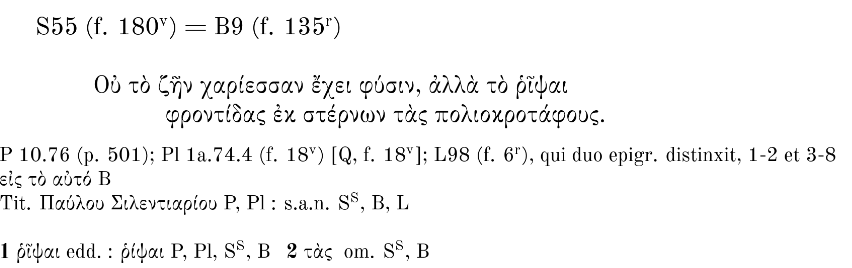
\includegraphics[width=4.16667in,height=1.5625in]{s55ekdosis.png}
\caption{ekdosis}
\end{figure}

et une en XML-TEI, qui donne le résultat suivant~:

\scriptsize
\begin{minted}{xml}
<div xml:id="div-edition_6" xml:lang="gr">
<div type="epigram" n="6">
  <head>
    <ref target="Ss1 #s2 #s3 #s4 #B #B1">S</ref>
    55 (f. 180<hi rend="sup">v</hi>) = <ref target="#B">B</ref>
    9 (f. 135<hi rend="sup">r</hi>)
  </head>
  <p>
    <note type="testium" target="#range(right(S55_1a),left(S55_2e))">
    <ref target="#P">P</ref> 10.76 (p. 501)</note>
    <note type="testium" target="#range(right(S55_1a),left(S55_2e))">
    <ref target="#Pl">Pl</ref> 1a.74.4 (f. 18<hi rend="sup">v</hi>) 
   [<ref target="#Q">Q</ref>, f. 18<hi rend="sup">v</hi>]</note>
    <note type="testium" target="#range(right(S55_1a),left(S55_2e))">
    <ref target="#l">L</ref>98 (f. 6<hi rend="sup">r</hi>), 
    qui duo epigr. distinxit, 1-2 et 3-8</note>
    <note type="lemmata" target="#range(right(S55_1a),left(S55_2e))">εἰς τὸ αὐτό 
    <ref target="#B">B</ref></note>
    <note type="tituli" target="#range(right(S55_1a),left(S55_2e))">
    Tit. Παύλου Σιλεντιαρίου <ref target="#P">P</ref>, 
    <ref target="#Pl">Pl</ref></note>
    <note type="tituli" target="#range(right(S55_1a),left(S55_2e))">
    s.a.n. <ref target="Ss1 #s2 #s3 #s4 #B,B1s1 #s2 #s3 #s4">S
    <hi rend="sup">S</hi></ref>, 
    <ref target="#B">B</ref>, <ref target="#l">L</ref></note>
    <anchor xml:id="S55_1a"/>
  </p>
  <lg type="hexdact">
    <l>Οὐ τὸ ζῆν χαρίεσσαν ἔχει φύσιν, ἀλλὰ τὸ 
    <app><lem source="#cramer_anecdota_1841,piccolos1 #s2 #s3,s4_s1 #s2 #s3,
    s4upplement_1853-1 #page_further_1981-2">ῥῖψαι</lem>
    <rdg wit="#P #Pl, Ss1 #s2 #s3 #s4 #B,B1s1 #s2 #s3 #s4 #B">ῥίψαι</rdg></app> </l>
    <l>φροντίδας ἐκ στέρνων 
    <app><lem>τὰς</lem><rdg wit="Ss1 #s2 #s3 #s4 #B,B1s1 #s2 #s3 #s4 #B"/></app> 
    πολιοκροτάφους. <anchor xml:id="S55_2e"/> </l>
  </lg>
</div>
</div>

\end{minted}
\normalsize

Cherchons à identifier les éléments principaux qui sont exprimés dans
ces manifestations matérielles des deux vers. Évidemment le modèle
textuel ici est bien plus complexe. Cela ne signifie pas que les
précédents étaient moins légitimes, juste qu'ils se concentraient sur un
nombre plus limité d'aspects. La délimitation du contexte était
différente. De ces aspects additionnels qui sont exprimés dans les
représentations qu'on vient de voir, il est nécessaire de préciser
qu'ils ne sont pas des notions abstraites qui se trouvent dans l'esprit
du philologue qui ensuite trouve une manière pour les incarner dans une
représentation matérielle. C'est plutôt le contraire~: ces aspects ne
peuvent exister que parce qu'il y en a une manifestation matérielle.
C'est l'existence de certaines syntaxes particulières, l'habitude du
philologue à les pratiquer -- à manipuler des éditions critiques, à les
produire -- qui fait en sorte qu'elles peuvent exister. C'est parce que
le format d'ekdosis me demande de renseigner une variante et offre une
incarnation syntaxique spécifique de la variante que l'idée même de
variante peut exister -- dans le sens spécifique qu'elle acquiert ici,
du moins -- et que je suis obligé de me poser la question des
différentes versions du texte dans des témoins différents\footnote{Pour
  une analyse cf Robert Alessi, {«\,Ekdosis: {Using} {LuaLaTeX} for
  producing compliant critical editions and highlighting parallel
  writings. {Special} {Issue} on {Collecting}, {Preserving}, and
  {Disseminating} {Endangered} {Cultural} {Heritage} for {New}
  {Understandings} through {Multilingual} {Approaches}\,»},
  \emph{Journal of Data Mining \& Digital Humanities}, 2020,
  \url{https://hal.archives-ouvertes.fr/hal-02779803} Estelle Debouy,
  {«\,Édition critique numérique avec le logiciel ekdosis pour
  {LuaLaTeX}. {L}'exemple des fragments latins d'atellanes\,»},
  \emph{Humanités numériques}, nᵒ 4, 2021}. La syntaxe pose des
questions, soulève des problèmes, oblige à donner des renseignements,
met devant des nécessités, des possibilités et des impossibilités. Une
annotation de Mathilde Verstraete en témoigne. Verstraete écrit (ligne
\ldots)~: «~\%alt = edd. ; devrais peut-être Declare a Short Hand plutôt
?~». En effet, la syntaxe ekdosis permet de produire des informations
sémantiques à propos des témoins qui sont déclarés dans le préambule et
ensuite appelés dans l'appareil critique. Cela n'est évidemment pas
possible en utilisant un logiciel comme Microsoft Word et Mathilde
Verstraete est en train de transcrire depuis une édition faite avec ce
logiciel par Lucia Floridi. Or, une annotation comme \texttt{edd.}
signifie que la variante est attestées dans les textes des éditeurs,
mais cela ne spécifie pas lesquels. Lucia Floridi entend donc, avec
cette annotation se référer au fait que tous les éditeurs intègrent une
correction évidente. Mais qu'est-ce que cela signifie d'un point de vue
sémantique~? Doit-on comprendre que la correction est présente dans
toutes les éditions~? Si c'est ainsi, pour traduire cette information en
balisage sémantique il est nécessaire de prendre une décision aux
implications théoriques fortes~: par exemple créer un groupe de témoins
déclarés comme ensemble dans le préambule -- une famille de
\texttt{Short\ hands}. La syntaxe ekdosis pose donc une question
épistémologique qui n'existe pas dans le format docx et qui doit être
traitée philologiquement.

Comme Robert Alessi le précise dans la documentation du paquet~:

\begin{quote}
\textbf{Terminology} Strictly speaking, the term ``witness'' should
apply to any manuscript evidence dating back to the Middle Ages used by
the editor to establish the edition text. That said, editors often
consult many other types of documents, such as modern editions,
articles, notes, correspondence and the like, all of which fall into the
category of ``sources''. Furthermore, unpublished conjectures are also
taken into account, not to mention the corrections and emendations that
are proposed in many places by the editor of the text. As it is
necessary to refer to scholars as individuals, ``scholars'' naturally
emerges as a third category. Any reference that is to be used in the
apparatus criticus must be ``declared'' in the preamble beforehand,
namely: manuscript sigla (either for single manuscripts or manuscript
families, primary or later hands, \&c.), abbreviated last names of
sources and scholars.\footnote{Robert Alessi, {«\,The ekdosis package.
  {Typesetting} {TEI}-xml compliant {Critical} {Editions}\,»}, novembre
  2021, \url{https://ctan.org/pkg/ekdosis}}
\end{quote}

Pour revenir au sens du texte dans ces trois manifestations, il faut,
par ailleurs, souligner un changement important de son sens~: il ne
s'agit plus de l'épigramme 76 du livre 10 de l'Anthologie Palatine, mais
de l'épigramme 55 de la \emph{Silloge Parisina} qui, comme nous le dit
l'appareil critique, correspond aux deux premiers vers de AP 10.76. Le
texte est donc pensé comme une tradition qui se transmet par des canaux
particuliers -- des manuscrits. Ce texte a donc des variantes. Cet
encodage montre qu'il n'y a pas une intention d'établir laquelle de ces
variantes est la «~bonne~», mais plutôt de rendre compte d'une tradition
multiple et hétérogène.

Il est important de souligner que le modèle originaire est celui de
l'encodage \LaTeX~ et que les deux autres sont dérivés. Et pourtant, si
on se concentre sur chacun des trois de façon séparée, nous pouvons
remarquer que la notion de texte qu'ils proposent est complètement
différente.

Pour résumer, l'encodage \LaTeX~ nous présente le texte comme une série
d'actions qui doivent se déclencher au moment de la lecture. Le texte
est donc une suite linéaire de symboles qui déclenchent des actions de
production de sens. L'ouverture du paragraphe, par exemple, avec la
commande \texttt{\textbackslash{}ekdiv} demande de faire des opérations
de mise en forme en ce qui concerne le format pdf -- et donc la sortie
mise en page --, demande aussi d'aller «~chercher~» dans le conspectus
siglorum la référence aux lettres qui constituent l'argument, demande
aussi de produire l'XML qui transforme ces informations en une série de
données exprimées dans un arbre XML.

L'idée de texte qui ressort du balisage XML est, au contraire, une idée
de données structurées dans une hiérarchie arborescente. Or ces deux
notions (le texte comme suite linéaire de symboles qui déclenchent une
action ou le texte comme ensemble de données structurées dans un arbre)
ne sont pas réductibles l'une à l'autre. La première est assez proche
d'une modélisation possible de la lecture d'un document~: le lecteur
avance et au fur et à mesure qu'il trouve des symboles qui sont
signifiants pour lui, il les met en relation et produit un sens et une
interprétation. Quand le lecteur voit ``L98'', ces symboles déclenchent
une action qui est celle de relier le texte qui suit au manuscrit qui a
été précédemment identifié avec la lettre L. La lecture continue, de
manière linéaire, et le mouvement des yeux -- qui passent d'un symbole à
l'autre, parfois se déplaçant dans la page, de l'appareil critique au
texte et \emph{vice versa} -- correspond à une série d'actions qui
produisent des relations et font émerger le sens. Le modèle de texte qui
ressort du balisage XML est complètement autre. Le texte n'est pas une
suite linéaire de caractères, mais une structure hiérarchique d'éléments
imbriqués dans un arbre. Il n'y a aucune linéarité et l'ensemble des
balises qui concernent un élément -- par exemple les variantes --
constituent une totalité de données non ordonnées de manière temporelle.
Ce modèle essaie de saisir le texte en tant que données, informations
objectives et qui expriment un sens qui leur est homothétique. Le sens
ne dérive pas du balisage, le sens \emph{est} le balisage. Dans le
modèle du XML-TEI, une série de caractères «~est une variante~» -- l'XML
produit une vision du texte qui consiste en des d'attributs ontologiques
--, alors que dans le modèle précédent, une série de caractères demande
des actions~: faire le lien avec un autre manuscrit qui porte un texte
différent.

Ces exemples démontrent deux principes qui sont au c\oe ur de la théorie
de l'édition que je propose ici. Le premier est que la matérialité du
texte est son sens et qu'il n'est pas possible d'imaginer une théorie du
texte qui fasse abstraction de cette matérialité. Le second est qu'il
n'est pas possible de trouver une modélisation du texte qui soit
universelle, car chaque configuration matérielle particulière donnera
lieu à un contexte d'observation déterminant non seulement un paradigme
épistémologique mais aussi une essence du texte. Il y aura donc
plusieurs essences du texte, non pas une ontologie, mais une
multiplicité d'ontologies.

Je vais essayer d'expliciter ces deux principes.

\hypertarget{le-cercle-de-la-moduxe9lisation}{%
\chapter{Le cercle de la
modélisation}\label{le-cercle-de-la-moduxe9lisation}}

\lettrine{L}e rapport entre théorie du texte et incarnation matérielle
du texte en un document peut être pensé comme un cas de modélisation. En
suivant la suggestion de Jean-Guy Meunier\footnote{Jean-Guy Meunier,
  {«\,Humanités numériques ou computationnelles : {Enjeux}
  herméneutiques\,»}, \emph{Sens Public}, décembre 2014,
  \url{http://www.sens-public.org/article1121.html}, consulté le 15
  octobre 2018 ; Jean-Guy Meunier, {«\,Humanités numériques et
  modélisation scientifique\,»}, \emph{Questions de communication}, nᵒ
  31, septembre 2017, p.~19‑48,
  \url{https://doi.org/10.4000/questionsdecommunication.11040}, consulté
  le 19 juin 2023}, nous pouvons donc identifier trois étapes de la
modélisation~: un modèle théorique, un modèle formel et un modèle
matériel. Selon cette approche, il y aurait d'abord une description
théorique du texte, faite en langage naturel~; ensuite une formalisation
de cette description en un langage non ambigu -- formel justement~; et
pour finir une implémentation matérielle du modèle formel.

Cette schématisation est proposée par Meunier -- en se basant notamment
sur les propositions de Willard McCarty\footnote{Willard McCarty,
  \emph{Humanities {Computing}}, Paperback edition, Basingstoke,
  Hampshire, Palgrave Macmillan, 2014} -- spécifiquement pour
l'implémentation numérique de modèles. Le modèle formel, dans le cas
spécifique d'une modélisation qui a comme but de produire une
implémentation matérielle en informatique, est un modèle numérique, dans
le sens qu'il est mathématique et fonctionnel. Le modèle formel, en
d'autres mots, consiste à transformer le modèle théorique en une série
d'entités discrètes et atomiques reliées entre elles par des fonctions
calculables. Or il me semble que l'on peut garder cette description de
la modélisation au delà des implémentations informatiques~: aussi quand
le modèle matériel vise d'autres supports -- notamment le papier.

Reprenons notre exemple précédent pour mieux expliquer ce concept. Selon
le schéma de Meunier, il y aurait d'abord un modèle
théorique\footnote{Elena Pierazzo se refère à cette première
  modélisation en l'appelant tout simplement «~théorie~» du texte. Cf.
  Elena Pierazzo, \emph{Digital {Scholarly} {Editing}: {Theories},
  {Models} and {Methods}}, London, Routledge, 2016,
  \url{https://doi.org/10.4324/9781315577227}.}. Dans notre premier
exemple~: ce texte est un distique élégiaque en grec, composé par deux
vers, un hexamètre et un pentamètre.

Ce modèle théorique doit ensuite être converti en modèle formel. Dans le
cadre d'un modèle formel destiné à une implémentation informatique, il
faudra transformer les affirmations précédentes en unités discrètes et
atomiques reliées par des fonctions. Donc par exemple~: on décrira comme
unité, le caractère grec, le vers, le pied, la langue et on aura ensuite
des relations qui définissent les interactions possibles parmi ces
unités. Cela nous permettra ensuite d'implémenter ce modèle fonctionnel
en un modèle matériel.

Mais on pourrait imaginer aussi un modèle formel dont l'objectif est
d'être implémenté dans un modèle matériel papier. Il faudra, dans ce cas
aussi, expliciter de façon formelle le modèle théorique. On n'aura pas
besoin de fonctions, mais toujours de définitions non ambigües pour
chaque élément utilisé. Par exemple~: un vers est une série de mots
isolés dans une ligne. Un mot est une série de caractères dont la
combinaison produit un sens\ldots{}

On en arrive au modèle matériel qui consiste en la manifestation
physique du texte. Notre épigramme sera donc quelque chose~: un fichier
\texttt{.txt} par exemple, ou un ficher \LaTeX~, ou un fichier XML-TEI,
ou un texte imprimé d'une certaine manière, avec une mise en page
spécifique.

Or cette description de la modélisation en trois étapes est sans doute
utile pour comprendre les différents aspects impliqués dans les modèles,
mais elle ne correspond pas à la réalité. Car aucun des modèles
théorique, formel ou matériel ne peut exister en tant que tel~; ils
existent seulement ensemble.

Un texte n'existe que dans sa matérialité située et c'est sa matière qui
contient le sens du texte formellement structuré. Les trois modèles n'en
font en réalité qu'un. Encore une fois l'idée selon laquelle la pensée
se ferait «~avant~» l'incarnation est complètement fausse. Cette idée,
pourtant, est très courante et très présente dans le monde de la
recherche en sciences humaines. Le grand chercheur imagine le modèle
théorique, fait à la limite une première ébauche du modèle formel et
laisse ensuite le travail «~trivial~» aux bras, aux mains sales qui
toucheront la matière. Mais la pensée est dans la matière et la
conviction du grand chercheur cache en réalité non pas une grande idée
théorique que les petites mains\footnote{Le concept de «~petites mains~»
  et la mise en question de cette pyramides de valeurs a été thématisée
  par Margot Mellet, en particulier dans Margot Mellet, {«\,Manifeste
  des petites mains {\textbar}\,»}, dans \emph{Blank.blue}, 2021,
  \url{https://blank.blue/meditions/manifeste-des-petites-mains/},
  consulté le 8 mars 2022 et Margot Mellet, \emph{. . et les doigts
  d'écrire se referment sur la paume {Recherche}-{Création} sur
  l'épaisseur de l'écriture}, thèse de doctorat, Université de Montréal,
  2024.} auront ensuite du mal à implémenter, mais juste une idée floue
-- quand il y en a une -- car ancrée sur une matérialité pauvre et mal
comprise, une idée vague qui devra ensuite être précisée par les petites
mains en question qui feront, elles, le travail de théorisation -- dont
le chercheur prendra à la fin la mérite, si c'est une réussite, ou pour
lequel il blâmera les petites mains si c'est un échec.

Il n'y a pas de sens en dehors de la matière. Encore une fois~: c'est la
matière qui pense.

La théorie se développe en manipulant la matière~; le modèle théorique
émerge lorsqu'on se heurte à une balise qu'on ne peut pas imbriquer, à
un format qui exprime un concept particulier d'une manière spécifique et
qui révèle ainsi l'incompatibilité logique et formelle entre deux
visions du texte, à la disposition des lignes dans une page et des mots
dans une ligne pour éviter une veuve ou un orphelin, à la facture d'une
police de caractères qui ne permet pas de voir la différence entre un
esprit et un accent.

Un modèle théorique riche est celui qui émerge d'une longue
manipulation. C'est la manipulation de la matière textuelle -- qu'elle
soit numérique ou papier -- qui fait voir les différents détails, les
cas particuliers, les exceptions, les incompatibilités, les
contradictions, les implications profondes. C'est cette manipulation qui
précise le modèle formel en délinéant les unités atomiques et les
relations qui les relient. Un modèle théorique qui ne passe pas par la
matière est en réalité juste un modèle théorique qui émerge d'une
manipulation paresseuse et trop rapide. La théorie abstraite est juste
une théorie très pauvre. Et pourtant combien de fois entend-on des
phrases comme «~moi, je m'occupe de la partie intellectuelle, le reste
je l'ai laissé à l'ingénieure~». Voilà, cette «~partie intellectuelle~»
est juste une manipulation paresseuse qui produit une théorie vague, une
pensée simpliste qui sera ensuite complexifiée, étoffée, enrichie par
l'ingénieure qui fera le vrai travail théorique, celui qui consiste à
laisser parler la matière pour essayer de comprendre comment elle pense.

Cette affirmation est difficile à démontrer et elle est surtout très
difficile à expliquer à ceux qui n'ont jamais fait ce type de travail.
Mais elle résultera évidente pour «~les petites mains~».

Un exemple pourra aider à mieux saisir ce que j'essaie d'exprimer.
L'histoire de la création du \emph{Pressoir}\footnote{Cf. Antoine
  Fauchié, Roch Delannay, Michael Sinatra et Marcello Vitali-Rosati,
  {«\,Exploring {New} ({Digital}) {Publishing} {Practices} with {Le}
  {Pressoir}\,»}, \emph{Pop! Public. Open. Participatory}, nᵒ 5,
  septembre 2023, \url{https://doi.org/10.54590/pop.2023.006}, consulté
  le 4 octobre 2023.} au sein de la Chaire de recherche sur les
écritures numériques à l'Université de Montréal. Le Pressoir est un
générateur de sites statiques pensé pour produire des livres savants
augmentés -- surtout en sciences humaines.

L'histoire commence en 2013, justement, avec une idée vague et un projet
de collection aux Presses de l'Université de Montréal~: la collection
Parcours numériques proposée par Michael Sinatra et moi-même. L'idée
vague, ou pour employer la terminologie utilisée ici, le modèle
théorique initial, est d'avoir une collection avec une double version~:
papier et numérique. La problématique qui nous animait était de
comprendre les relations possibles entre édition numérique et édition
papier. Nous essayons de comprendre quel allait être le futur du
livre\footnote{Cf. Le futur du livre~:
  https://blog.sens-public.org/marcellovitalirosati/le-futur-du-livre/}
à une époque où la discussion était particulièrement polarisée~: d'une
part, les «~progressistes~» qui envisageaient un «~passage~» total au
numérique, en considérant les environnements numériques comme
«~meilleurs~», plus expressifs et plus puissants et, de l,autre, les
«~réactionnaires~» qui faisaient l'éloge du papier en voyant dans le
numérique un appauvrissement ou du moins une menace à la riche tradition
du papier.

L'intuition à la base de notre démarche était d'imaginer au contraire
une complementarité entre les deux modèles en essayant d'identifier les
caractéristiques, les forces et les faiblesses de l'un et de l'autre et
en les mettant en dialogue au lieu de les mettre en compétition. Le
papier devait épouser une des caractéristiques que le support semble
mieux implémenter, à savoir la linéarité. Comme le remarque notamment
Vandendorpe\footnote{Christian Vandendorpe, \emph{Du papyrus à
  l'hypertexte: essai sur les mutations du texte et de la lecture},
  Paris, La Découverte, 1999,
  \url{http://vandendorpe.org/papyrus/PapyrusenLigne.pdf}}, différents
supports sont caractérisés par un niveau différent de linéarité. À
partir d'un support très linéaire, comme le papyrus, fait pour être
déroulé en rendant très peu ergonomique un aller-retour entre
différentes parties du texte, en passant par le codex, dont la structure
en pages avec une numérotation permet une certaine indexation -- une
table des matières et des index qui rendent possible de sauter d'un
passage à l'autre --, jusqu'à l'hypertexte qui est pensé -- à partir
d'intuitions comme celle du Memex de Vannevar Bush\footnote{Vannevar
  Bush, {«\,As we may think\,»}, \emph{Atlantic Magazine}, 1945,
  \url{http://www.theatlantic.com/magazine/archive/1945/07/as-we-may-think/303881/}
  T. H. Nelson, {«\,Complex {Information} {Processing}: {A} {File}
  {Structure} for the {Complex}, the {Changing} and the
  {Indeterminate}\,»}, dans \emph{Proceedings of the 1965 20th
  {National} {Conference}}, New York, NY, USA, ACM, coll. «~{ACM} '65~»,
  1965, p.~84‑100, \url{https://doi.org/10.1145/800197.806036}, consulté
  le 9 janvier 2015 et Alain Mille, {«\,D'{Internet} au web\,»}, dans
  éd. Marcello Vitali-Rosati et Michael Sinatra, \emph{Pratiques de
  l'édition numérique}, Les Ateliers de {[}sens public{]}, 2014,
  consulté le 25 octobre 2024 pour une histoire du Memex et de son
  rapport avec le web.} -- pour permettre une tabularité très poussée.
L'«~intertextualité~», si on veut l'appeler ainsi, des hypertextes est
loin d'une idée abstraite et vague de «~liens~» entre les textes, elle
est matérielle, elle est faite d'hyperliens qui permettent concrètement
de transformer des passages de texte ou des mots en unités atomiques
auxquelles le lien peut se référer. Cette matérialité peut déjà être
identifiée dans les premières idées de Bush, qui propose la notion de
lien à partir des possibilités techniques qu'il connaissait en 1945~:
des microfilms, lus par une machine, avec la possibilité mécanique
d'enregistrer une position spécifique du lecteur pour pouvoir ensuite la
rappeler. Cette idée \emph{matérielle} changera ensuite de forme~; en
HTML, une balise -- par exemple un
\texttt{\textless{}span\textgreater{}texte\textless{}/span\textgreater{}}
peut avoir un identifiant qui est exprimé en tant qu'attribut -- par
exemple
\texttt{\textless{}span\ id="1"\textgreater{}texte\textless{}/span\textgreater{}}
auquel le lien peut se référer -- avec une syntaxe du type
\texttt{\textless{}a\ href="\#1"\textgreater{}texte\ du\ lien\textless{}/a\textgreater{}}.
Une référence de ce type est matériellement impossible dans un support
papier -- du moins dans les syntaxes normalement utilisées. Un index
peut se référer à une page, mais non à un mot.

À partir de ce constat -- qui, comme l'exemple le montre, est loin
d'être désincarné, même s'il se fonde sur une manipulation textuelle
très superficielle, qui ne rentre pas dans les milliers de détails
possibles, mais qui se limite à regarder la matérialité d'une des
macrostructures du format HTML et du format «~livre papier~» --, l'idée
de Parcours numériques était d'avoir, pour chaque livre, une version
linéaire et une version tabulaire. La version linéaire devait essayer de
radicaliser l'idée de linéarité: le papier n'aurait pas contenu toutes
les structures tabulaires qu'il contient normalement, comme les notes de
bas de page, les références bibliographiques et l'appareil critique en
général, justement parce que ces structures sont peu adaptées au
support. La version numérique, au contraire, devait radicaliser l'idée
de tabularité en multipliant les renvois infratextuels, l'ajout
d'appareil critique, la mise à disposition de parcours de lecture
alternatifs.

Le pari était de proposer non pas deux versions alternatives, mais deux
versions complémentaires, permettant une double lecture. Une qui
permette de saisir la thèse du livre en suivant une argumentation
linéaire -- comme un roman -- et l'autre qui suggère une lecture d'étude
et d'approfondissement d'un sujet, en laissant les thèses et
l'argumentation du livre sur le fond.

Mais ces deux modèles théoriques du texte, justement parce que basés sur
une analyse légère des modèles matériels, restait très pauvre. L'idée a
commencé à se préciser lors des premières implémentations -- pour la
version numérique la construction d'une plateforme réalisée avec le CMS
Spip\footnote{Nous avions considéré d'autres possibilité, dont Scalar,
  une plateforme créée dans le but de produire des livres augmentés.
  Mais les contraintes des autres plateformes s'adaptaient mal à notre
  idée initiale et la possibilité de personnaliser Spip nous avait
  semblé nous donner plus de liberté.} par Aurélie Veyron-Churlet, pour
la version papier la réalisation des premiers livres, lors mise en page,
le travail avec les auteurs pour imaginer avec eux un texte savant sans
appareil critique.

Concentrons-nous sur la version numérique. L'usage de Spip était une
manière de déléguer le modèle théorique aux possibilités
d'implémentation proposées par ce CMS -- évidemment avec un travail
d'adaptation. Spip fonctionne avec une base de données relationnelle
assez classique, sur le principe de la plupart des CMS des années 2000.
Le balisage infratextuel est assez limité, car justement
l'implémentation en base de données relationnelle n'est pas compatible
avec la structure à arbre typique par exemple d'un document XML.

La collection a vu le jour et les premiers livres ont été publiés en
2014. En éditant les textes augmentés, en collaboration avec Hélène
Beauchef, l'éditrice qui s'occupe de la version numérique, nous avons
vite réalisé que le modèle théorique que Spip nous proposait était trop
pauvre~: nous nous sommes heurtés aux caractéristiques figés du modèle
matériel que nous avions adopté. C'est là que nous avons réalisé que la
seule manière de développer un modèle théorique riche pour un «~livre
augmenté~» était de commencer à toucher à la matérialité du texte, à
bricoler, à mettre, donc, les mains à la pâte.

En même temps, nous avons lancé un projet éditorial parallèle, les
\emph{Ateliers de Sens public} avec une idée semblable qui aurait pu
ensuite être mutualisée pour la collection des \emph{Ateliers} et pour
celle de Parcours numériques. Le travail, commencé avec Hélène Beauchef,
Servanne Monjour et Nicolas Sauret, a débuté en repartant d'un balisage
textuel flexible, qui nous permettait, au fur et à mesure des besoins,
de spécifier les structures formelles dont nous avions besoin. Le choix
des formats markdown (pour le texte), yaml (pour les métadonnées) et
bibtex (pour la bibliographie) a semblé une bonne piste. La combinaison
de ces trois formats est largement utilisée en sciences humaines, en
particulier par une large communauté qui s'est créée autour du
convertisseur Pandoc. Il est intéressant de remarquer que Pandoc a été
créé par John McFarlane, un philosophe qui l'a développé justement pour
répondre à ses propres besoins de gestion du texte, des besoins proches
des nôtres qui voulions justement modéliser des textes en sciences
humaines.

Markdown a donc été utilisé en se basant sur l'idée de se servir de
Pandoc comme convertisseur pour produire du HTML. La syntaxe markdown
est ainsi employée dans sa version \emph{pandoc flavored}. Cela permet
notamment de créer des classes \emph{ad hoc} pour baliser des contenus,
classes qui sont ensuite transformées en classes HTML. Yaml permet de
créer des métadonnées qui s'expriment avec une structure de type
clé-valeur -- par exemple \texttt{titre:\ Texte\ du\ titre}. C'est une
syntaxe très légère, excellente pour la modélisation, car on peut créer
n'importe quel jeu de métadonnées tout simplement en écrivant du plein
texte. Si besoin d'une clé de plus, on n'a qu'à la rajouter.

Nous avons pu commencer à préciser notre modèle théorique en définissant
dans le texte des structures qui devaient être indexées, en produisant
des modèles formels pour définir les «~contenus additionnels~», etc.

Notre possibilité de modélisation était fortement liée à nos
connaissances informatiques~: nous n'arrivions à imaginer que les
possibilités que nous étions concrètement capables d'implémenter. Au
début, notre littératie était assez limitée. Nous avons commencé avec
des scripts bash qui mettaient ensemble une série de logiciel de bas
niveau, comme \texttt{awk}, \texttt{sed}, ou un préprocesseur comme
pp\footnote{https://github.com/CDSoft/pp} qui permettait d'appliquer
certaines macros à la syntaxe du markdown, ainsi qu'un gabarit de mise
en forme, créé par Edward Tufte et implémenté par Dave
Liepmann\footnote{Cf. https://www.daveliepmann.com/}.

Notre idée de ce que devait être le texte augmenté et notre modèle
théorique étaient directement issus de la matérialité de ces formats et
logiciels et ils évoluaient au fur et à mesure que nos compétences de
manipulation augmentaient.

Finalement, le script bash a été transformé en un script python, bien
plus complexe. Un développeur, David Larlet, a rejoint l'équipe, ainsi
qu'un certain nombre de doctorants -- parmi lesquels Antoine Fauchié et
Roch Delannay. Les capacités de manipulation et l'expérience de
traitement d'un nombre de publication croissant, nous a permis, à chaque
itération, de complexifier le modèle, jusqu'à arriver à un livre
augmenté qui pouvait être considéré comme généralisable. Ce n'était plus
le modèle qui pouvait fonctionner pour le cas particulier de livre que
nous étions en train de publier, mais un modèle théorique qui pouvait
décrire une série assez large de livres augmentés. Un modèle théorique
qui pouvait donc être partagé car il décrivait un artefact bien
spécifié, formalisé, à la structure claire et réutilisable.

Qui a conçu ce modèle théorique~? Qui a produit le sens~? Qui a pensé?
Cette idée a émergé dans le travail collectif de manipulation de
formats, outils, langages de programmation, textes numériques
particuliers, protocoles de versionnage, algorithmes\ldots{} Ce qui est
à l'origine de l'émergence du modèle théorique n'est pas une personne,
mais une série de dynamiques complexes qui comprennent des échanges, des
formations, la prise en main d'outils et d'environnements numériques
particuliers, la collaboration au sein d'un laboratoire dans lequel
jouent un rôle fondamental aussi la matérialité de l'institution, avec
ses spécificités, ces lieux, ces caractéristiques économiques,
culturelles, techniques, etc.\footnote{Margot Mellet parle du café, par
  exemple https://blank.blue/conf/crihn/} La théorie n'est pas venue
d'un individu qui pense, mais elle a émergé des caractéristiques
physiques de la matière. Encore une fois~: c'est la matière qui pense.

Accepter l'impossibilité de séparer les trois étapes de la modélisation
et surtout d'imaginer une hiérarchie qui mettrait le modèle théorique au
dessus -- du point de vue de sa valeur symbolique -- du modèle formel et
du modèle matériel a trois conséquences majeures, deux qui concernent
spécifiquement la théorie du texte et la théorie de l'édition et une
dernière qui a une portée plus large que l'on peut facilement
caractériser de métaphysique.

En premier lieu, comme nous l'avons vu, il n'est pas possible d'imaginer
la réduction de la multiplicité des modèles à une unité. Dit autrement,
il n'est pas possible de se poser, avec De Rose et al.~la question
\emph{What is text, really}? Ce fameux article de 1990 a été un des
points de départ du XML, en proposant l'idée du texte comme Ordered
Hierarchy of Content Objects (OHCO). Or, si cette idée et son
implémentation dans les différents langages XML est sans doute une
interprétation très riche de ce que peut être un texte et si elle répond
à des besoins herméneutiques communs à plusieurs approches de lecture en
science humaines, elle ne peut pas être considérée la \emph{seule}
possible, ni la \emph{meilleure}. Elle est, elle-aussi, située et
contextuelle. Comme nous l'avons montré, certaines conceptions du texte
ne peuvent y être réduites.

Une deuxième conséquence de nos considérations peut être aussi comprise
comme une critique à l'approche de De Rose et plus précisément à l'idée
qu'il est nécessaire, pour produire un modèle théorique riche du texte,
de séparer sa structure sémantique de ses caractéristiques
présentationnelles. Selon cette idée, la force des approches OHCO serait
le fait de se concentrer sur le \emph{sens} du texte et d'ignorer
l'incarnation matérielle de ce sens dans une forme particulière. C'est
l'idée notamment de séparer de manière nette le balisage sémantique du
traitement présentationnel\footnote{Citer Elena}. D'un côté des balises
qui expriment ce que le texte signifie, de l'autre un dispositif qui
permet de «~rendre~» ce sens avec une incarnation graphique. Pour faire
un exemple~: on peut exprimer qu'une série de caractères constitue un
titre de niveau un -- par exemple avec la balise HTML
\texttt{\textless{}h1\textgreater{}} -- et ensuite traiter cette
information de manière graphique ailleurs -- par exemple dans un fichier
CSS qui nous dira qu'il faut mettre ce titre en gras et dans une police
de caractère plus grande. Cette approche est sans doute d'un grand
intérêt. Elle est \emph{une} bonne modélisation. Comme tous les modèles,
elle permet de délimiter et définir précisément le geste
d'interprétation en incluant certains aspect et en en excluant d'autres.
Mais elle n'est pas la seule légitime. Il serait en effet tout autant
légitime de se concentrer sur l'aspect graphique comme aspect
signifiant. C'est ce qui arrive, par exemple, lorsqu'on réalise une
édition diplomatique. Cela est évidemment possible en restant dans une
approche OHCO, et il y a notamment des spécifications de schémas XML qui
se concentrent sur ces aspects. Mais, et c'est le plus important, il ne
faut pas se leurrer et croire que la séparation du balisage en
sémantique et présentationnel corresponde à une véritable séparation
d'un sens immatériel par rapport à une incarnation matérielle de ce sens
en un rendu quelconque. Car le balisage sémantique est lui aussi une
incarnation située et présentationnelle du texte. Lorsqu'on manipule les
balises, de fait, on manipule un artefact matériel, avec une syntaxe
spécifique, avec des mises en forme de cette syntaxe qui souvent ne sont
que présentationnels -- que l'on pense à l'indentation, par exemple,
sans laquelle la syntaxe XML n'aurait aucun sens, du moins pour une
personne qui essayerait de la produire ou de la lire.

Même l'approche OHCO est donc fortement matérielle. Il ne s'agit pas
d'une structure abstraite. Pour être plus précis~: le sens du mot
«~abstraction~» est toujours relatif. Faire abstraction signifie mettre
entre parenthèses un aspect que l'on ne veut pas considérer, justement
pour pouvoir se concentrer sur la manipulation des autres aspects
matériels qui nous intéressent et qui risqueraient de rendre trop
complexe notre manipulation du texte. L'abstraction, loin d'être une
tentative de saisir l'immatérialité, est un effort qui permet
d'accroître la matérialité des éléments sur lesquels on se concentre en
rendant possible que leur matérialité se révèle de manière encore plus
forte.

\hypertarget{mais-alors-quest-ce-quun-uxeatre-humain}{%
\chapter{Mais alors qu'est ce qu'un être
humain~?}\label{mais-alors-quest-ce-quun-uxeatre-humain}}

\lettrine{C}omme je l'annonçais, il y a une troisième implication de nos
réflexions, une conséquence ontologique fondamentale, peut-être celle
qui explique la réticence à embrasser une vision véritablement
matérialiste du monde.

La production de sens est, en effet, la caractéristique fondamentale sur
laquelle on fonde la définition de l'humain. L'être humain serait le
producteur de la pensée. C'est ce qui, traditionnellement, permet de
distinguer les humains de toutes les autres choses, et, en même temps,
de les mettre au dessus d'elles. L'être humain de Platon dans le
\emph{Phèdre} est l'entité qui, parce qu'elle est liée de façon
privilégiée à l'immatérialité, s'élève au dessus des autres choses du
monde en se rapprochant des dieux. L'être humain des chrétiens, fait à
l'image de Dieu, est, lui aussi, l'être qui se détache de l'immanence
matérielle pour accéder à la transcendance~: de cette manière il se
trouve au dessus de toutes les autres choses du monde. La rhétorique de
l'immatérialité est un dispositif de production de hiérarchies
ontologiques.

Ces hiérarchies permettent à la fois de distinguer les humains des
autres animaux et de toutes les autres «~choses du monde~», mais aussi
de déterminer qui est plus humain parmi les humains en mettant donc en
place la production d'une élite qui s'oppose au reste des individus. Si
l'essence de l'humain est de partager l'immatérialité qui caractérise ce
qu'il y a de plus élevé ontologiquement, alors il y aura des humains
plus humains que d'autres~: des élites qui se rapprochent plus de
l'immatérialité, des subalternes qui sont du côté de la matière et des
autres choses inhumaines -- des formats, des protocoles, des supports,
des techniques, des conditions économiques, etc.

Mais que se passe-t-il si ce paradigme est renversé? Que se passe-t-il
si c'est la matière qui pense~? Les hiérarchies ontologiques tombent et
tout se retrouve sur un même plan immanent. Tout d'abord, s'écroule la
hiérarchie entre les élites et les subalternes, entre les grands auteurs
et les petites mains, entre le philosophe et sa secrétaire. Mais, si on
assume radicalement les conséquences de notre raisonnement, même la
démarcation entre humain et non humain commence à vaciller. Car à la
production du sens participent au même titre des individus, des formats,
des algorithmes, des objets, au point où il n'est plus possible de
tracer une séparation nette. Les contours même des agents producteurs de
sens sont floutés. Qui a pensé quoi~? Est-ce moi~? Est-ce nous~? Est-ce
cette balise, cette feuille, cet écran, ce cigare~? Qui est qui~?

Prendre au sérieux le fait que la matière pense, prendre au sérieux le
fait qu'il faut bien parler d'une théorie de l'édition et non seulement
de pratiques éditoriales signifie mettre en question la possibilité
d'une définition stable de l'humain. En suivant la suggestion de Karen
Barad, il faut arrêter d'essayer de saisir l'essence de l'humain et
s'intéresser plutôt aux dynamiques qui font en sorte que certaines
définitions émergent dans certaines conditions particulières. Au lieu de
se demander~: «~qu'est-ce que l'humain~», il faut se demander «~pourquoi
a-t-on défini l'humain ainsi dans ce contexte~?~».

La définition de l'humain, plus qu'être un point de départ, quelque
chose de donné, sera le résultat d'un contexte particulier. Les humains
ne sont plus les producteurs de sens, mais les produits d'un contexte
matériel. L'auteur n'est pas le producteur du sens d'un texte, mais son
produit. L'auteur émerge des dynamiques matérielles qui font le texte.

Cette idée est au centre des réflexions de ce qu'on appelle les
\emph{posthuman studies}, une série d'approches et théories qui essayent
de mettre en question une notion forte et bien définie d'humain. Le sens
du mot post-humanisme doit ici être précisée car il peut porter à
confusion. On pourrait en effet interpréter cette notion comme une
tentative d'aller au delà de l'humain en «~augmentant~» des
caractéristiques qui lui seraient essentielles et propres. C'est ce que
proposent notamment les transhumanistes. Dans leur idée il s'agit
d'identifier les aspects spécifiques de l'humain et de les rendre encore
plus forts en s'appuyant notamment sur les technologies. Le
post-humanisme a l'objectif opposé. Pour le dire avec les mots de Carry
Wolfe~:

\begin{quote}
posthumanism in my sense isn't posthuman at all --- in the sense of
being ``after'' our embodiment has been transcended --- but is only
posthumanist, in the sense that it opposes the fantasies of
disembodiment and autonomy, inherited from humanism itself.a Cary
Wolfe\footnote{\emph{What is posthumanism?}, Minneapolis, University of
  Minnesota Press, coll. «~Posthumanities series~», v. 8, 2010}
\end{quote}

Plus qu'aller «~au delà~» de l'humain il s'agit de remonter en deçà
d'une définition stable d'humain. Plus précismént, dans le texte de
Wolfe, mais aussi, dans un autre des livres fondateurs de ce mouvement,
celui de Rose Braidotti\footnote{Rosi Braidotti, \emph{The posthuman},
  Cambridge, UK ; Malden, MA, USA, Polity Press, 2013}, il est question
de s'opposer à l'idée de l'être humain désincarné et au centre de
l'univers qui serait proposée notamment par l'humanisme.

Or il me semble que ces auteurs se trompent d'objectif polémique quand
ils considèrent l'humanisme comme responsable d'une idée forte,
désincarnée et bien définie de l'humain. En réalité l'humanisme, comme
le souligne bien Eugenio Garin a eu une fonction opposée dans la
conception de l'humain. Car l'humanisme a été d'abord et avant tout une
critique radicale de l'essence humaine telle que définie dans la
tradition scolastique et plus en général chrétienne. Pour les humanistes
on ne peut plus penser l'humain comme une brique centrale de la
structure métaphysique dont la cohérence est garantie par Dieu. Pour les
humanistes, on ne peut plus fonder la définition de l'humain sur la base
de la ressemblance à Dieu, ce qui lui garantirait une place centrale
dans l'Univers. Les humanistes au contraire approchent l'humain de
manière immanente et donc incarnée, en se concentrant sur ce qui est à
la porté de notre espèce. Au lieu de s'appuyer sur une prétendue essence
qui serait fondée sur une structure métaphysique préexistante, il faut
regarder ce qui fait partie de notre immanence. L'objet de l'étude ne
sont donc plus «~les grandes cathédrales d'idées~», mais les textes et
les artefacts culturels en tant qu'ils sont -- à différence de la
métaphysique -- à mesure d'homme, et donc aussi incarnés.

Cette attitude me semble tout à fait cohérente avec mon propos~:
abandonner une pyramide de valeurs qui se fonde sur des présupposées
métaphysiques et revenir à la matérialité de l'immanence.

L'humanisme est loin de l'outrecuidance anthropocentrique dont
l'accusent Wolfe et Braidotti, il est plutôt l'humble acceptation de la
contingence humaine. L'homme n'est pas au centre de l'univers, il
devient juste la seule mesure possible, car on n'a pas de système
ontologique garanti par une transcendance divine.

Garin le souligne en analysant les critiques qui ont été portées à la
philosophie humaniste, comme philosophie faible, qui a perdu de vue les
grands enjeux de la métaphysiques scolastique~:

\begin{quote}
Perché ciò di cui si lamenta da tante parti la perdita è proprio quello
che gli umanisti vollero distrutto, e cioè la costruzione delle grandi
«cattedrali di idee», delle grandi sistemazioni logico-teologiche: della
Filosofia che sussume ogni problema, ogni ricerca al problema teologico,
che organizza e chiude ogni possibilità nella trama di un ordine logico
prestabilito. A quella Filosofia, che viene ignorata nell'età
dell'umanesimo come vana ed inutile, si sostituiscono indagini concrete,
definite, precise, nelle due direzioni delle scienze morali (etica,
politica, economica, estetica, logica, retorica) e delle scienze della
natura per capire la vibrazione con cui Valla dinanzi alla parola, al
verbum, richiama al fatto che ci troviamo innanzi a un puro mezzo di
comunicazione, cosa certo grandissima, ma umana. Eugenio
Garin\footnote{\emph{L'umanesimo italiano. {Filosofia} e vita civile nel
  {Rinascimento}}, 7 edizione, Roma, Laterza, 1994}
\end{quote}

La compréhension de l'humanisme comme d'un mouvement qui véhiculerait
une conception forte de l'humain et qui mettrait une idée désincarnée
d'humain au centre est en réalité un mythe romantique. Ce mythe est
souvent lié, dans notre imaginaire à une icône précise~: celle de
l'homme vitruvien de Léonard de Vinci\footnote{Foglio 228 du Gabinetto
  Disegni e Stampe delle Gallerie dell'Accademia di Venezia.} qui est
d'ailleurs souvent évoquée dans les critiques post-humanistes, jusqu'à
être proposée, en version détournée dans la couverture du livre de
Braidotti.

Il me semble donc important, pour clore ma démonstration, de revenir à
cette icône pour déconstruire l'idée d'être humain au centre du monde à
laquelle elle a pu être reliée.

Le dessin est souvent présenté comme une géniale tentative de Léonard de
proposer une idée d'être humain parfait\footnote{Cf. pour ne citer que
  quelques exemples Emanuele Lugli, {«\,In cerca della perfezione.
  {Nuovi} elementi per l'{Uomo} vitruviano di {Leonardo} da {Vinci}\,»},
  dans éd. Francesca Borgo, \emph{Leonardo e {Vitruvio}. {Oltre} il
  cerchio e il quadrato}, Venezia, Marsilio, 2019, p.~69‑91 ; Paola
  Salvi, Leonardo, Accademia di Belle Arti di Brera et Regia Accademia
  di Belle Arti (dir.), \emph{Approfondimenti sull'{Uomo} vitruviano di
  {Leonardo} da {Vinci}: atti delle giornate di studi, {Accademia} di
  {Belle} {Arti} di {Brera}, {Sala} {Napoleonica}, 9 febbraio 2010, 4 -
  5 maggio 2011}, Poggio a Caiano, CB Edizioni, 2012 ; Paola Salvi,
  {«\,L'{Uomo} vitruviano: il piede, il centro del corpo, il dibattito
  {Bossi}/{Verri} e una copia di {Andrea} {Appiani}\,»}, dans éd. Paola
  Salvi, \emph{Leonardo da {Vinci} e l'{Accademia} di {Brera7}}, Silvana
  Editoriale, 2020 ; Pierre Gros, Paolo Clini et Daniela Amadei,
  {«\,Vitruvio e {Leonardo}, le geometrie platoniche "nell'uomo dalla
  bella forma" ({De} {Architectura} {III}, 1, 2-3)\,»}, ITA, 2013,
  \url{https://iris.univpm.it/handle/11566/128680}, consulté le 16
  octobre 2024.}~: le corps inscrit dans un cercle, une série de
proportions mathématiques harmonieuses qui révèlent de quelle manière
l'humain est la réalisation parfaite d'un projet rationnel de la nature.
D'une certaine manière, l'homme vitruvien serait donc une reformulation
humaniste des structures métaphysiques médiévales~: une essence forte et
stable qui n'est plus garantie par Dieu, mais par les mathématiques qui
régissent, comme des idées platoniciennes, un nouveau édifice
métaphysique.

Or cette lecture est tout simplement fausse, elle est une
réinterprétation romantique de Léonard et du dessin, basée sur
uneidéalisation et sur une rhétorique immatérielle qui ignore -- ou en
tout cas sousestime -- le fait que le dessin est d'abord une
représentation graphique -- et on pourrait presque dire un commentaire
-- d'une série de passages précis d'un texte, le \emph{De architectura}
de Vitruve.

Le dessin est le croquis d'un lecteur qui essaie de bien comprendre son
\emph{auteur}. La relecture romantique invente la figure du grand génie,
Léonard, qui produit une idée nouvelle, inédite et révolutionnaire,
Léonard en tant qu'individu qui produit la pensée, mais cette figure
n'est pas une réalité historique, mais une retroprojection.

Les raisons souvent évoquées pour appuyer ces interprétations sont le
fait que les proportions représentées par Léonard ne correspondent pas à
celles de Vitruve et que donc Léonard donne une lecture originale et
créative du texte. Léonard créerait sa propre idée d'homme parfait.

Or, comme le démontre Francesco Paolo Di Teodoro\footnote{Je suis ici
  débiteur de deux articles Francesco Paolo Di Teodoro, {«\,Vetruvio
  architecto mecte nella sua op(er)a d'architectura che lle misure
  dell'omo {[}...{]}: filologia del testo e inciampi vitruviani nel
  foglio 228 di {Venezia}\,»}, dans éd. Annalisa Perissa Torrini,
  \emph{Leonardo da {Vinci} l'uomo modello del mondo}, Cinisello
  Balsamo, Milano, Silvana Editoriale, 2019, p.~35‑41 et Francesco Paolo
  Di Teodoro, {«\,Leonardo e {Vitruvio}: "de homine bene figurato''\,»},
  \emph{Achademia Leonardi Vinci}, 3, nᵒ 3, décembre 2023, p.~33‑62,
  \url{https://doi.org/10.6093/2785-4337/10620}, consulté le 4 janvier
  2024 outre que plusieurs conversations privées.}, cette interprétation
se base sur une abstraction du texte de Vitruve réel dont pouvait
disposer Léonard. Les interpolations de Léonard ont été identifiées en
confrontant son texte avec l'édition critique de Vitruve, un texte
idéal, reconstruit par les philologues bien plus tard et que Léonard ne
pouvait donc pas lire. Il est intéressant que cette fausse démarche
d'interprétation se fonde sur une idéalisation du texte de Vitruve qui
permet ensuite une idéalisation du travail de Léonard~: un texte
abstrait donc, qui ne se touche pas, un texte imperceptible et de
l'autre côté un génie créateur qui produit du sens à partir de rien.
Cette idéalisation est par ailleurs contraire au valeurs mêmes qui
émergent à l'époque de Léonard, où voient le jour les premières
approches philologiques et où on commence justement à se poser la
question de la matérialité des textes et de l'origine des documents --
que l'on pense à la fameuse donation de Constantin.

Les textes, pour les humanistes, sont bien matériels et le sens émerge
de document et de manipulations concrètes. Certaines interpolations sont
dues donc à l'édition dont disposait Léonard. Léonard, loin d'essayer
d'être original, a simplement devant les yeux une édition particulière
de Vitruve, avec des erreurs. D'autres interpolations de Léonard sont
des déductions évidentes du texte de Vitruve (comme le calcul de
correspondance entre des mesures) ou des petites erreurs de Léonard
(comme le rapport entre \emph{cubiti} et \emph{passi}). Il n'invente
rien, il ne veut pas du tout proposer quelque chose d'innovant. Il n'est
pas en train d'essayer de définir l'essence parfaite de l'homme. Il veut
tout simplement comprendre le texte qu'il a devant les yeux et il le
fait en dessinant. Le croquis, loin d'être le chef-d'œuvre de
l'intelligence humaine qui arrive à saisir sa propre essence, est juste
le travail d'un lecteur qui ai besoin de manipuler un texte et de le
représenter graphiquement pour en saisir le sens.

Tombent ici l'idée de Léonard comme grand génie et l'idée de l'humanisme
comme période qui essaye de mettre l'homme au centre du monde.

Léonard n'est pas l'auteur, il est juste le produit de certains textes~:
le \emph{De architectura}, mais non pas dans une version idéale du
texte, mais dans une édition précise qu'il avait sous les yeux. Et
l'humain, loin d'être le centre du monde, est ce qui ressort des textes.

L'idée de l'humanisme est que ce sont les textes qui définissent
l'humain et qu'il n'y a pas quelque chose comme l'humain qui serait
définit par un dessin divin qui le placerait au centre de l'univers,
mais plutôt une humanité qui ressort des textes. L'humanitas -- en
restant dans la tradition cicéronienne dont la redécouverte par
Petrarque constitue justement le début de l'humanisme -- est l'étude des
lettres, et ces lettres sont des textes matériels.

La convergence entre une vision de ce type et l'émergence de la presse à
caractères mobiles n'est pas un hasard. L'humanisme peut être considéré
comme un moment de retour à la matérialité.

Je propose donc de revenir à ces idées, d'oublier les \emph{doxai}
immatérielles des romantiques et des post-structuralistes, de produire
une véritable théorie de l'édition, de laisser de côté les mythes des
grands individus, d'abandonner les hiérarchies symboliques et
ontologiques.

Cela implique aussi d'abandonner une idée d'être humain forte et stable
et réfléchir plutôt à comment les frontières qui distinguent l'humain
d'autre chose se stabilisent et se déstabilisent dans des contextes
particulier.

C'est la matière qui pense, et cela nous oblige à repenser le rôle des
textes, des formats, de l'édition et des êtres humains. C'est la matière
qui pense, l'édition devient une véritable philosophie.

\hypertarget{bibliographie}{%
\chapter{Bibliographie}\label{bibliographie}}

\hypertarget{refs}{}
\begin{CSLReferences}{1}{0}
\leavevmode\vadjust pre{\hypertarget{ref-Alessi2020b}{}}%
\textsc{Alessi} Robert, {«\,Ekdosis: {Using} {LuaLaTeX} for producing
compliant critical editions and highlighting parallel writings.
{Special} {Issue} on {Collecting}, {Preserving}, and {Disseminating}
{Endangered} {Cultural} {Heritage} for {New} {Understandings} through
{Multilingual} {Approaches}\,»}, dans \emph{Journal of Data Mining \&
Digital Humanities}, 2020,
\url{https://hal.archives-ouvertes.fr/hal-02779803}.

\leavevmode\vadjust pre{\hypertarget{ref-ekdosis}{}}%
---------, {«\,The ekdosis package. {Typesetting} {TEI}-xml compliant
{Critical} {Editions}\,»}, novembre 2021,
\url{https://ctan.org/pkg/ekdosis}, tex.version: 1.4.

\leavevmode\vadjust pre{\hypertarget{ref-archibald_texte_2009}{}}%
\textsc{Archibald} Samuel, \emph{Le texte et la technique : {La} lecture
à l'heure des médias numériques}, s. l., Le Quartanier, 2009.

\leavevmode\vadjust pre{\hypertarget{ref-barad_meeting_2007}{}}%
\textsc{Barad} Karen, \emph{Meeting the {Universe} {Halfway}: {Quantum}
{Physics} and the {Entanglement} of {Matter} and {Meaning}}, Durham,
Duke University Press Books, 2007.

\leavevmode\vadjust pre{\hypertarget{ref-braidotti_posthuman_2013}{}}%
\textsc{Braidotti} Rosi, \emph{The posthuman}, Cambridge, UK ; Malden,
MA, USA, Polity Press, 2013.

\leavevmode\vadjust pre{\hypertarget{ref-bush_as_1945}{}}%
\textsc{Bush} Vannevar, {«\,As we may think\,»}, dans \emph{Atlantic
Magazine}, 1945,
\url{http://www.theatlantic.com/magazine/archive/1945/07/as-we-may-think/303881/}.

\leavevmode\vadjust pre{\hypertarget{ref-Debouy2021a}{}}%
\textsc{Debouy} Estelle, {«\,Édition critique numérique avec le logiciel
ekdosis pour {LuaLaTeX}. {L}'exemple des fragments latins
d'atellanes\,»}, dans \emph{Humanités numériques}, nᵒ 4, 2021.

\leavevmode\vadjust pre{\hypertarget{ref-derrida_pharmacie_1968}{}}%
\textsc{Derrida} Jacques, {«\,La pharmacie de {Platon}\,»}, dans
\emph{Tel Quel}, nᵒ 32,33, 1968, OCLC: 494339475.

\leavevmode\vadjust pre{\hypertarget{ref-di_teodoro_vetruvio_2019}{}}%
\textsc{Di Teodoro} Francesco Paolo, {«\,Vetruvio architecto mecte nella
sua op(er)a d'architectura che lle misure dell'omo {[}...{]}: filologia
del testo e inciampi vitruviani nel foglio 228 di {Venezia}\,»}, dans
éd. Annalisa Perissa Torrini, \emph{Leonardo da {Vinci} l'uomo modello
del mondo}, p.~35‑41, Cinisello Balsamo, Milano, Silvana Editoriale,
2019.

\leavevmode\vadjust pre{\hypertarget{ref-di_teodoro_leonardo_2023}{}}%
---------, {«\,Leonardo e {Vitruvio}: "de homine bene figurato''\,»},
dans \emph{Achademia Leonardi Vinci}, 3, nᵒ 3, décembre 2023, p.~33‑62,
\url{https://doi.org/10.6093/2785-4337/10620}, consulté le 4 janvier
2024, Number: 3.

\leavevmode\vadjust pre{\hypertarget{ref-fauchie_exploring_2023}{}}%
\textsc{Fauchié} Antoine, \textsc{Delannay} Roch, \textsc{Sinatra}
Michael et \textsc{Vitali-Rosati} Marcello, {«\,Exploring {New}
({Digital}) {Publishing} {Practices} with {Le} {Pressoir}\,»}, dans
\emph{Pop! Public. Open. Participatory}, nᵒ 5, septembre 2023,
\url{https://doi.org/10.54590/pop.2023.006}, consulté le 4 octobre 2023,
Publisher: CISP Press.

\leavevmode\vadjust pre{\hypertarget{ref-friedrich_stern_2003}{}}%
\textsc{Friedrich} Bretislav et \textsc{Herschbach} Dudley, {«\,Stern
and {Gerlach}: {How} a {Bad} {Cigar} {Helped} {Reorient} {Atomic}
{Physics}\,»}, dans \emph{Physics Today}, 56, nᵒ 12, décembre 2003,
p.~53‑59, \url{https://doi.org/10.1063/1.1650229}, consulté le 10 avril
2024.

\leavevmode\vadjust pre{\hypertarget{ref-garin_umanesimo_1994}{}}%
\textsc{Garin} Eugenio, \emph{L'umanesimo italiano. {Filosofia} e vita
civile nel {Rinascimento}}, Roma, Laterza, 1994.

\leavevmode\vadjust pre{\hypertarget{ref-gros_vitruvio_2013}{}}%
\textsc{Gros} Pierre, \textsc{Clini} Paolo et \textsc{Amadei} Daniela,
{«\,Vitruvio e {Leonardo}, le geometrie platoniche "nell'uomo dalla
bella forma" ({De} {Architectura} {III}, 1, 2-3)\,»}, ITA, 2013,
\url{https://iris.univpm.it/handle/11566/128680}, consulté le 16 octobre
2024, Accepted: 2015-04-07T18:55:04Z.

\leavevmode\vadjust pre{\hypertarget{ref-lugli_cerca_2019}{}}%
\textsc{Lugli} Emanuele, {«\,In cerca della perfezione. {Nuovi} elementi
per l'{Uomo} vitruviano di {Leonardo} da {Vinci}\,»}, dans éd. Francesca
Borgo, \emph{Leonardo e {Vitruvio}. {Oltre} il cerchio e il quadrato},
p.~69‑91, Venezia, Marsilio, 2019.

\leavevmode\vadjust pre{\hypertarget{ref-mccarty_humanities_2014}{}}%
\textsc{McCarty} Willard, \emph{Humanities {Computing}}, Basingstoke,
Hampshire, Palgrave Macmillan, 2014.

\leavevmode\vadjust pre{\hypertarget{ref-mellet_manifeste_2021}{}}%
\textsc{Mellet} Margot, {«\,Manifeste des petites mains {\textbar}\,»},
dans \emph{Blank.blue}, 2021,
\url{https://blank.blue/meditions/manifeste-des-petites-mains/},
consulté le 8 mars 2022.

\leavevmode\vadjust pre{\hypertarget{ref-mellet__2024}{}}%
---------\emph{. . . et les doigts d'écrire se referment sur la paume
{Recherche}-{Création} sur l'épaisseur de l'écriture}, Thèse de
doctorat, Université de Montréal, 2024.

\leavevmode\vadjust pre{\hypertarget{ref-meunier_humanites_2014}{}}%
\textsc{Meunier} Jean-Guy, {«\,Humanités numériques ou computationnelles
: {Enjeux} herméneutiques\,»}, dans \emph{Sens Public}, décembre 2014,
\url{http://www.sens-public.org/article1121.html}, consulté le 15
octobre 2018.

\leavevmode\vadjust pre{\hypertarget{ref-meunier_humanites_2017}{}}%
---------, {«\,Humanités numériques et modélisation scientifique\,»},
dans \emph{Questions de communication}, nᵒ 31, septembre 2017, p.~19‑48,
\url{https://doi.org/10.4000/questionsdecommunication.11040}, consulté
le 19 juin 2023, ISBN: 9782814303256 Number: 31 Publisher: Presses
universitaires de Nancy.

\leavevmode\vadjust pre{\hypertarget{ref-mille_internet_2014}{}}%
\textsc{Mille} Alain, {«\,D'{Internet} au web\,»}, dans éd. Marcello
Vitali-Rosati et Michael Sinatra, \emph{Pratiques de l'édition
numérique}, Les Ateliers de {[}sens public{]}, 2014, consulté le 25
octobre 2024.

\leavevmode\vadjust pre{\hypertarget{ref-nelson_complex_1965}{}}%
\textsc{Nelson} T. H., {«\,Complex {Information} {Processing}: {A}
{File} {Structure} for the {Complex}, the {Changing} and the
{Indeterminate}\,»}, dans \emph{Proceedings of the 1965 20th {National}
{Conference}}, p.~84‑100, New York, NY, USA, ACM, coll. «~{ACM} '65~»,
1965, \url{https://doi.org/10.1145/800197.806036}, consulté le 9 janvier
2015.

\leavevmode\vadjust pre{\hypertarget{ref-pierazzo_digital_2016}{}}%
\textsc{Pierazzo} Elena, \emph{Digital {Scholarly} {Editing}:
{Theories}, {Models} and {Methods}}, London, Routledge, 2016,
\url{https://doi.org/10.4324/9781315577227}.

\leavevmode\vadjust pre{\hypertarget{ref-salvi_luomo_2020}{}}%
\textsc{Salvi} Paola, {«\,L'{Uomo} vitruviano: il piede, il centro del
corpo, il dibattito {Bossi}/{Verri} e una copia di {Andrea}
{Appiani}\,»}, dans éd. Paola Salvi, \emph{Leonardo da {Vinci} e
l'{Accademia} di {Brera7}}, Silvana Editoriale, 2020.

\leavevmode\vadjust pre{\hypertarget{ref-salvi_approfondimenti_2012}{}}%
\textsc{Salvi} Paola, \textsc{Leonardo}, \textsc{Accademia di Belle Arti
di Brera} et \textsc{Regia Accademia di Belle Arti} (dir.),
\emph{Approfondimenti sull'{Uomo} vitruviano di {Leonardo} da {Vinci}:
atti delle giornate di studi, {Accademia} di {Belle} {Arti} di {Brera},
{Sala} {Napoleonica}, 9 febbraio 2010, 4 - 5 maggio 2011}, Poggio a
Caiano, CB Edizioni, 2012.

\leavevmode\vadjust pre{\hypertarget{ref-vandendorpe_du_1999}{}}%
\textsc{Vandendorpe} Christian, \emph{Du papyrus à l'hypertexte: essai
sur les mutations du texte et de la lecture}, Paris, La Découverte,
1999, \url{http://vandendorpe.org/papyrus/PapyrusenLigne.pdf}.

\leavevmode\vadjust pre{\hypertarget{ref-wolfe_what_2010}{}}%
\textsc{Wolfe} Cary, \emph{What is posthumanism?}, Minneapolis,
University of Minnesota Press, coll. «~Posthumanities series~», v. 8,
2010.

\end{CSLReferences}
